\documentclass[tikz,crop]{standalone}

% Part of the preamble, for TikZ figures.
% This is used in both the main document and in the subfigures.
% One exception is minted: since the path depends on the file, it is not set.
\usepackage{tikz}
\usepackage{xcolor}
\usepackage{pgfplots}

\pgfplotsset{compat=1.18}
\usepgfplotslibrary{statistics}

\usetikzlibrary{shapes,arrows,positioning,backgrounds,calc,intersections,calc}

\definecolor{ugent-re}{RGB}{220, 78, 40}        % vermilion			/ vermiljoen
\definecolor{ugent-we}{RGB}{45, 140, 168}       % no match
\definecolor{ugent-ge}{RGB}{232, 94, 113}       % rose				/ bleekrood
\definecolor{ugent-ea}{RGB}{111, 113, 185}      % distant blue		/ verblauw
\definecolor{ugent-pp}{RGB}{251, 126, 58}       % deep orange		/ dieporanje
\definecolor{ugent-ps}{RGB}{113, 168, 96}       % yellow green		/ geelgroen

\tikzstyle{python}=[fill=ugent-ps!50!white]
\tikzstyle{java}=[fill=ugent-we!50!white]
\tikzstyle{haskell}=[fill=ugent-ea!50!white]
\tikzstyle{js}=[fill=ugent-pp!50!white]
\tikzstyle{c}=[fill=ugent-re!50!white]

\newlength{\block}
\setlength{\block}{0.75cm}

\tikzstyle{a}=[anchor=north west]
\tikzstyle{box}=[a,draw,rectangle]
\tikzstyle{node}=[a,draw,minimum height=0.5cm,align=center,fill=white,text depth=.25ex]
\tikzstyle{document}=[node,tape,tape bend top=none]
\tikzstyle{cont}=[box,minimum height=1\block,minimum width=1\block]
\tikzstyle{arrow}=[draw, -latex]
\tikzstyle{inner}=[box,draw=gray]

% Blue box style
\tikzstyle{bluebox}=[draw=ugent-we,java]
\tikzstyle{redbox}=[draw=ugent-re,c]
\tikzstyle{greenbox}=[draw=ugent-ps,python]

% Some things specific to TESTed imagery.
\tikzstyle{tc}=[box,draw=ugent-ps]
\tikzstyle{comp}=[box,draw=ugent-re,fill=ugent-re,fill opacity=0.05]
\tikzstyle{exec}=[box,draw=ugent-we,fill=ugent-we,fill opacity=0.10]

% Stuff from tested-engine/concept.tex
\tikzstyle{process}=[node,rectangle]
\tikzstyle{terminator}=[node,rectangle,rounded corners=0.5cm]
\tikzstyle{io}=[node,trapezium,trapezium left angle=70,trapezium right angle=-70,minimum width=2.5cm,trapezium stretches=true]
\tikzstyle{small}=[font=\footnotesize,color=darkgray]
\tikzstyle{submission}=[document,align=right,minimum width=3cm,minimum height=1cm,text depth=0.5cm,inner sep=0.5mm,font=\scriptsize]

% Stuff from chatper3/flow.tex
\tikzstyle{height}=[minimum height=0.75\block]
\tikzstyle{contt}=[cont,minimum height=0.75\block]
\tikzstyle{compop}=[comp,text opacity=1]
\tikzstyle{execop}=[exec,text opacity=1]

\tikzstyle{hnode}=[draw,anchor=center,minimum height=\block,text depth=.25ex,align=center]
\tikzstyle{executable}=[hnode,ultra thick,fill=gray!10]
\tikzstyle{inner-exec}=[node,anchor=center,minimum width=3.25\block,densely dotted,font=\footnotesize,fill=none]
\tikzstyle{stmt}=[node,anchor=center,fill=gray!30,minimum width=4.5\block,font=\footnotesize]
\tikzstyle{fieldset}=[minimum height=\block,fill=white,text depth=.5ex,fill=white]

% Minted environments for use in Tikz
\newminted[tikzjava]{java}{autogobble,linenos=false,fontsize=\tiny,stripall}
\newminted[tikzpython]{python}{autogobble,linenos=false,fontsize=\tiny,stripall}
\newminted[tikztext]{text}{autogobble,linenos=false,fontsize=\tiny,stripall}


\begin{document}

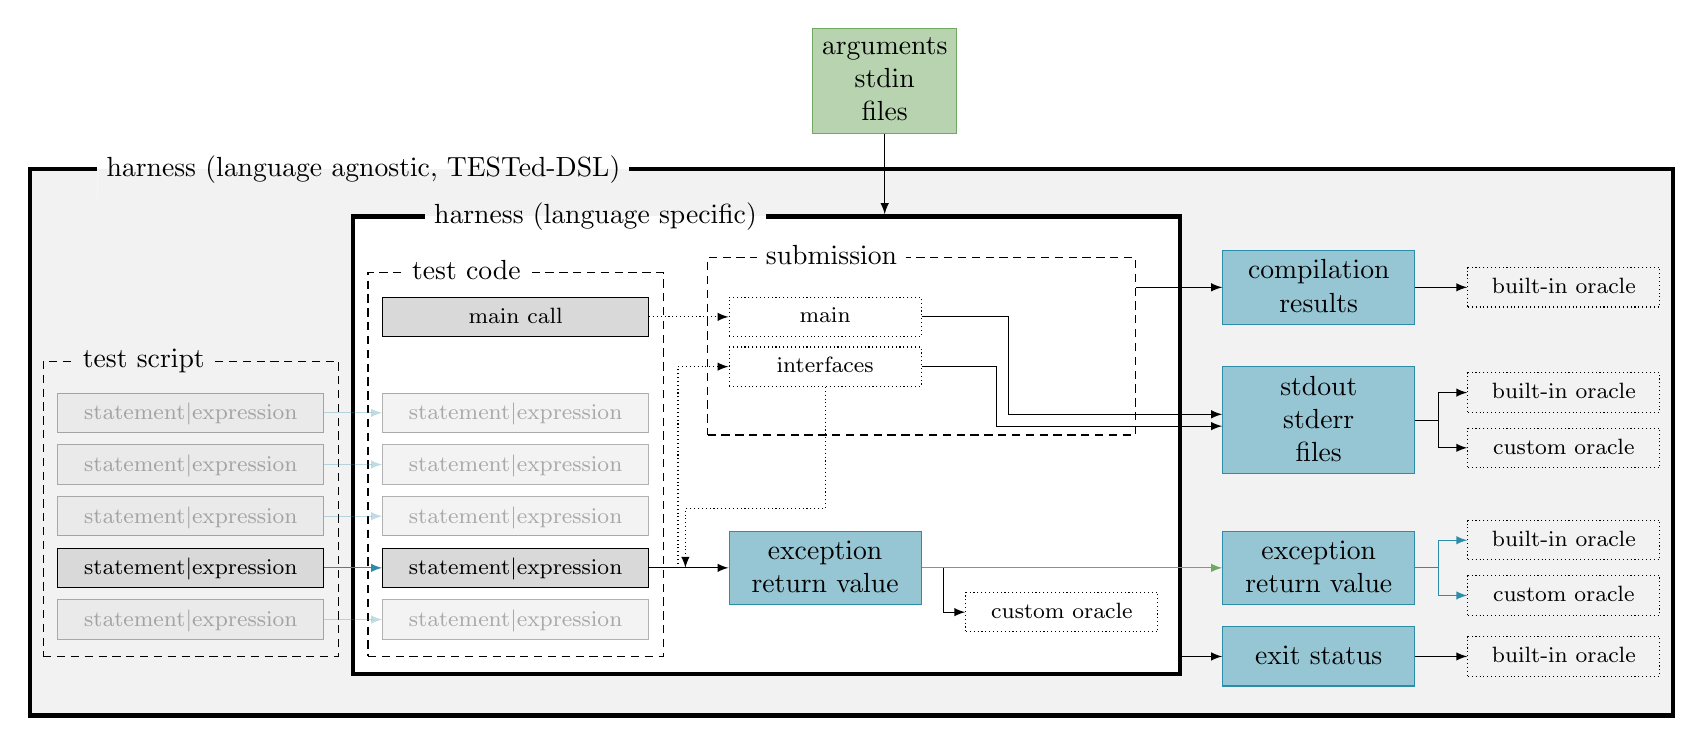
\begin{tikzpicture}[x=0.75cm,y=0.75cm,fill fraction/.style={path picture={
  \fill[#1]
  (path picture bounding box.west) rectangle
  (path picture bounding box.south east);
}},
  fill fraction/.default=gray!50]

  \node[executable,ultra thick,label={[fieldset,above left=-0.54\block and 3.75\block,fill fraction=gray!10]harness (language agnostic, TESTed-DSL)},minimum width=27.825\block,minimum height=9.25\block] at (7.4375,3.875) (tested) {};

  \node[inner-exec,densely dashed,anchor=center,fill=none,minimum width=5\block,minimum height=5\block,label={[fieldset,above left=-0.52\block and -0.4\block,fill=gray!10]test script}] at (-3.75,2.75) (testscout) {};

  \node[stmt,opacity=0.3] at (testscout|-0,4.375) (testsco1) {statement\textbar{}expression};
  \node[stmt,opacity=0.3] at (testscout|-0,3.5) (testsco2) {statement\textbar{}expression};
  \node[stmt,opacity=0.3] at (testscout|-0,2.625) (testsco3) {statement\textbar{}expression};
  \node[stmt] at (testscout|-0,1.75) (testsco4) {statement\textbar{}expression};
  \node[stmt,opacity=0.3] at (testscout|-0,0.875) (testsco5) {statement\textbar{}expression};


  \node[hnode,fill=white,ultra thick,label={[fieldset,above left=-0.54\block and 0mm,fill=gray!10,fill fraction=white]harness (language specific)},minimum width=14\block,minimum height=7.75\block] at (6, 3.825) (harness) {};

  \node[inner-exec,densely dashed,anchor=center,fill=none,minimum width=5\block,minimum height=6.5\block,label={[fieldset,above left=-0.52\block and -0.25\block]test code}] at (1.75,3.5) (testsc) {};

  \node[stmt] at (testsc|-0,6) (mainc) {main call};

  \node[stmt,opacity=0.3] at (testsc|-0,4.375) (testsc1) {statement\textbar{}expression};
  \node[stmt,opacity=0.3] at (testsc|-0,3.5) (testsc2) {statement\textbar{}expression};
  \node[stmt,opacity=0.3] at (testsc|-0,2.625) (testsc3) {statement\textbar{}expression};
  \node[stmt] at (testsc|-0,1.75) (testsc4) {statement\textbar{}expression};
  \node[stmt,opacity=0.3] at (testsc|-0,0.875) (testsc5) {statement\textbar{}expression};

  \draw[arrow,draw=ugent-we,opacity=0.3] (testsco1) -- (testsc1);
  \draw[arrow,draw=ugent-we,opacity=0.3] (testsco2) -- (testsc2);
  \draw[arrow,draw=ugent-we,opacity=0.3] (testsco3) -- (testsc3);
  \draw[arrow,draw=ugent-we] (testsco4) -- (testsc4);
  \draw[arrow,draw=ugent-we,opacity=0.3] (testsco5) -- (testsc5);

  \node[inner-exec,densely dashed,minimum width=7.25\block,minimum height=3\block,label={[fieldset,above left=-0.52\block and 0.25\block]submission}] at (8.625,5.5) (subm) {};

  \node[inner-exec, anchor=center,below left=0mm and 0mm of subm.center,fill=none,minimum width=3.25\block] (interface) {interfaces};

  \node[inner-exec, anchor=center,fill=none,minimum width=3.25\block] at (interface|-mainc) (main) {main};
  \draw[arrow,densely dotted] (mainc) -- (main);

  \node[hnode,minimum width=3.25\block,bluebox] at (interface|-testsc4) (out) {exception\\return value};
  \draw[arrow] (testsc4) -- (out);

  \draw[arrow,densely dotted] (out-|4.5,0) |- (interface);

  \draw[arrow,densely dotted] (interface) |- (out|-0,2.75) -| (out-|4.625,0);

  \node[inner-exec] at (11,1) (cor) {custom oracle};

  \draw[arrow] (out) -| (cor.west-|9,0) -- (cor);

  \node[hnode,minimum width=3.25\block,bluebox] at (15.35,0|-testsc4) (oout) {exception\\return value};
  \node[hnode,minimum width=3.25\block,bluebox] at (oout|-0,6.5) (oout1) {compilation\\results};
  \node[hnode,minimum width=3.25\block,bluebox] at (oout|-0,4.25) (oout2) {stdout\\stderr\\files};
  \node[hnode,minimum width=3.25\block,bluebox] at (oout|-0,0.25) (oout3) {exit status};

  \draw[arrow,draw=ugent-ps] (out) -- (oout);
  \draw[arrow] (subm.east|-oout1) -- (oout1);

  \draw[arrow] (interface) -| (9.90,4.15) -- (oout2.west|-0,4.15);
  \draw[arrow] (main) -| (10.10,4.35) -- (oout2.west|-0,4.35);

  \draw[arrow] (harness.east|-oout3) -- (oout3);

  \node[inner-exec] at (19.5,0|-oout1) (built1) {built-in oracle};
  \draw[arrow] (oout1) -- (built1);

  \node[inner-exec,above=0.125\block] at (built1|-oout2) (built2) {built-in oracle};
  \node[inner-exec,below=0.125\block] at (built1|-oout2) (cust2) {custom oracle};

  \draw[arrow] (oout2) -| (built2.west-|17.375,0) -- (built2);
  \draw[arrow] (oout2) -| (cust2.west-|17.375,0) -- (cust2);

  \node[inner-exec,above=0.125\block] at (built1|-oout) (built3) {built-in oracle};
  \node[inner-exec,below=0.125\block] at (built1|-oout) (cust3) {custom oracle};

  \draw[arrow,draw=ugent-we] (oout) -| (built3.west-|17.375,0) -- (built3);
  \draw[arrow,draw=ugent-we] (oout) -| (cust3.west-|17.375,0) -- (cust3);

  \node[inner-exec] at (built1|-oout3) (built3) {built-in oracle};
  \draw[arrow] (oout3) -- (built3);

  \node[hnode,minimum width=2\block,greenbox] at (8,10) (in) {arguments\\stdin\\files};
  \draw[arrow] (in) -- (harness.north-|in.south);

\end{tikzpicture}

\end{document}
